\section{Test Environment}
\label{sec:testenv}
To comply with the need for continuously running multiple experiments on new proposed algorithms as well as existing algorithms, a test environment framework has been designed and implemented.

The test environment made it easy to reuse existing models, algorithms and experiments as a part of new algorithms and models. 
The algorithms we propose are mainly based on the well known \gls{baum-welch}, and hence the test environment aims to provide a flexible use of \gls{baum-welch}, to reduce code redundancy.
The architecture of the test environment is depicted in figure \ref{fig:testenvironment}.

\begin{figure}[!htb]
\centering
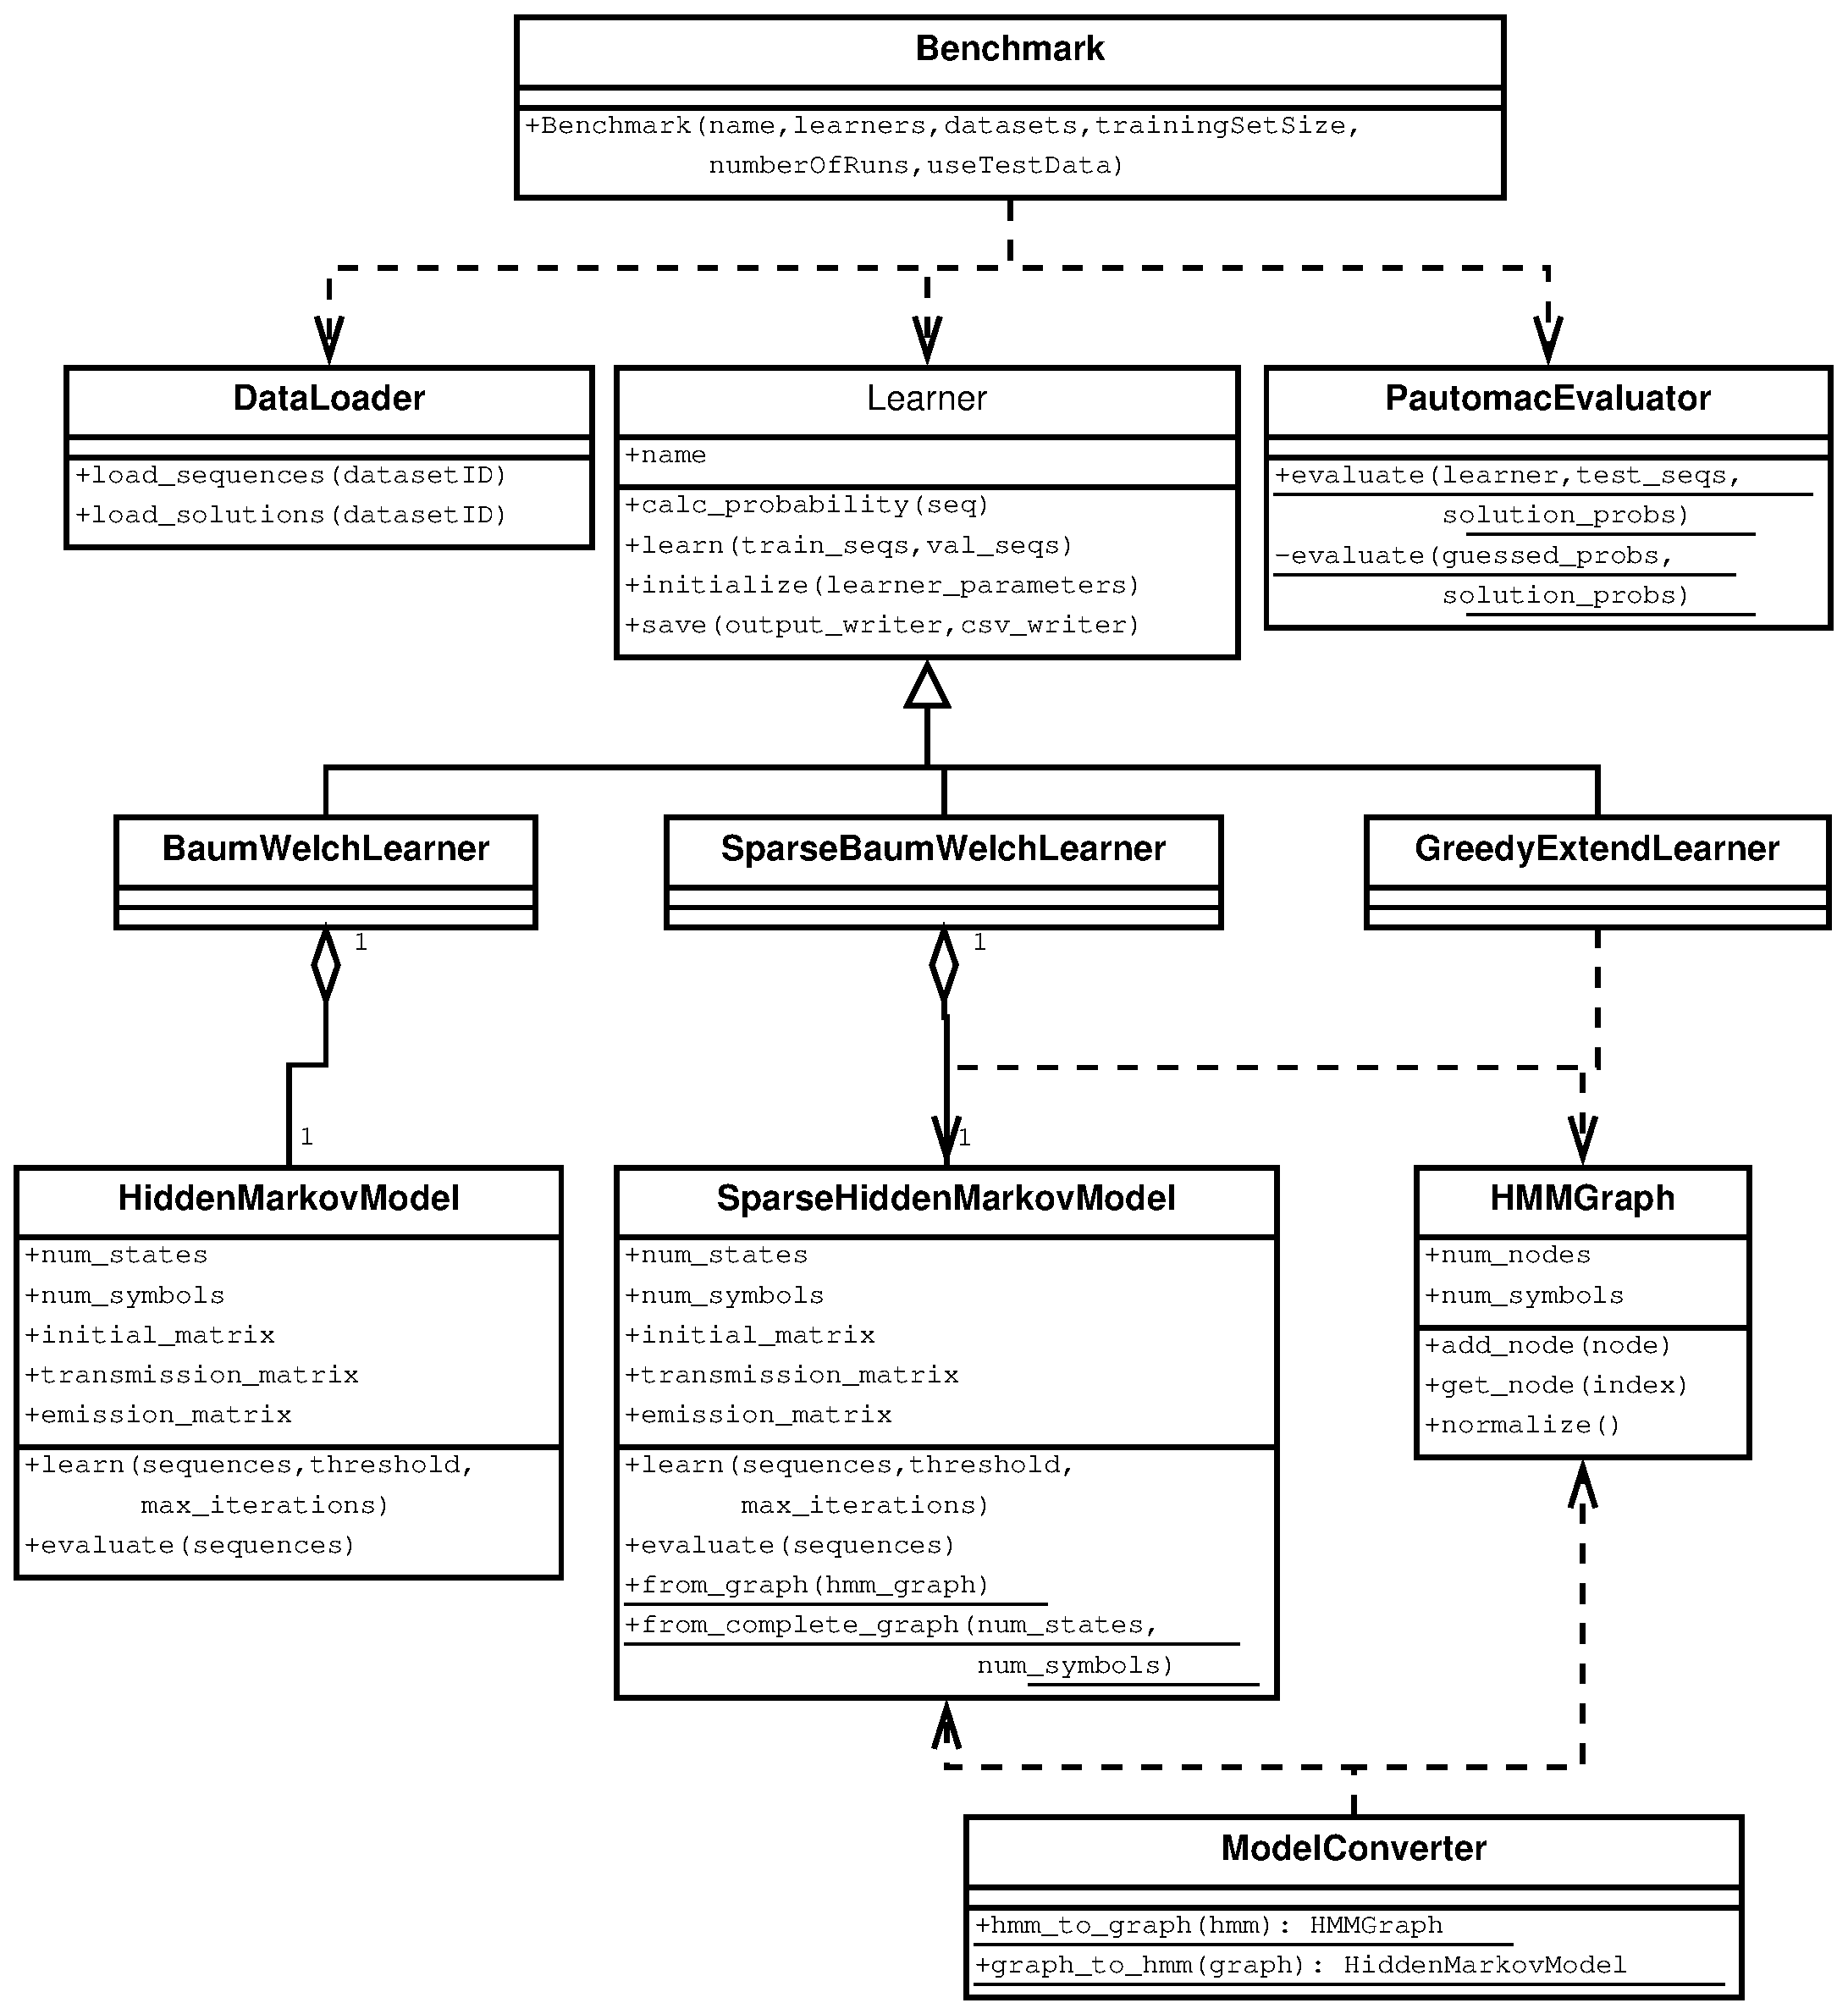
\includegraphics[scale=.4]{pictures/test-environment-overview.eps}
\caption{An overview of the test environment architecture.}
\label{fig:testenvironment}
\end{figure}

\subsection{Benchmark}
The \formatclass{Benchmark} class is the core element of the test environment as it is responsible for executing and tracking the actual tests and recording the results. The \formatclass{Benchmark} class is first initialised by specifying the parameters for the tests to be run and subsequently, the initialized tests are executed by calling the \formatfunction{Run} method.

The test parameters needed to perform a Benchmark:

\begin{itemize}
	\item[] Name: This is the name of the folder created by the benchmarking process, where all the results are stored.
	\item[] Learners: A list of all learners that should be benchmarked.
	\item[] Datasets: A list of integers, representing the IDs of the \emph{PAutomaC} problem sets to benchmark on. The \formatclass{Benchmark} class loads this data using the \formatclass{DataLoader}.
	\item[] Number of runs: By using an increased number of runs, an average can be taken to produce a more reliable result.
	\item[] Training and validation set size: The training data loaded from the \emph{PAutomaC} train data file is split into a training and validation set of the specified sizes.
	\item[] Evaluate on test data: If true, the score of each learner is calculated according to the \emph{PAutomaC} evaluation criteria by using the test data from the competition. If false, the log likelihood of the validation data is returned.
\end{itemize}

Beside the parameters required by the benchmarker, each learner can determine that additional parameters need to be specified for that particular learner. For instance these parameters could allow for the user to specify a range and a step size, for how a test should be executed.

While benchmarking, the \formatclass{Benchmark} class outputs information about its current state through the command line. Its current state covers the current run, learner, and dataset. After the benchmark has finished, it saves the results of the benchmark in two different formats: a plaintext format that ensures easy readability and a \gls{csv} format to allow easy data management for other applications or analysis. The saved data includes the configuration tested as well as data about the score and running time for the learner's different runs. For the dynamical algorithms (those that continuously extend a model), the benchmarker also saves intermediate data about the performance of each of the intermediate models encountered. 
Finally, a summary is saved for each learner to show the average and median performance over the different runs for each configuration and the best performing configuration is highlighted. A global summary through all the learners is also offered, comparing their best configurations. Last but not least the intermediate learned models are saved for every run, learner and configuration such that a review is possible if one wants to reason about the models while learned.

All of the results are updated in real time so that if the benchmark fails to finish successfully, at least partial results from the already finished experiments are available. In many cases, it can be relevant to examine only partial results, which may help one decide whether to continue the test or stop it and conduct a new experiment using more promising parameters.

\subsection{Data}
The \formatclass{DataLoader} class is responsible for loading training data, test data and solution data from the files published at the \emph{PAutomaC} website. Both training and test data contain a list of sequences, while the solution data contains a list of probabilities, one for each test sequence, representing the probability of the generating that particular sequence from the model used. However, the probabilities are normalized, so they sum to 1.

The data loader stores the loaded data in an entity class called \formatclass{DataSet} passed to the \formatclass{Benchmark}. The \formatclass{DataSet} is responsible for splitting the loaded training data obtained from \emph{PAutomaC} data files into data for training and for validation. The split is done in a pseudo-random fashion in order to ensure that multiple algorithms in different configurations will be tested on the same training and validation data, but also provide diversity through increased number of runs, where a different shuffle is generated for each run.

As mentioned, the test environment also allows for specification of a given number of sequences to be used as training or validation data. It thus becomes possible to run tests on smaller training sets in cases where only fast, approximate result is required.

\subsection{PautomacEvaluator}
The \formatclass{PautomacEvaluator} class is responsible for computing the score of a learner by either of the two offered evaluation criteria. As earlier mentioned, the criteria are either the \emph{PAutomaC} evaluation criterion described in section \ref{sec:pautomac}, which compares the probabilities calculated by the learner directly to the solution file, or by logarithmic likelihood of the validation data, that is, how likely it is, that the learned model have generated the sequences used as validation data.

\subsection{Learner}
An integral part of the test environment is the abstract class \formatclass{Learner}. The \formatclass{Learner} provides a common interface for every implemented learning algorithm allowing the \formatclass{Benchmark} and \formatclass{PautomacEvaluator} to work with every learning approach indifferently.

The \formatclass{Learner} class specifies several methods that are implemented by individual learning algorithms and are subsequently called by either the \formatclass{Benchmark} class or the \formatclass{PautomacEvaluator} class:

\begin{itemize}
	\item[] \formatfunction{initialize(learner\_parameters)} -- initialises the \formatclass{Learner} into a given configuration. As different learning algorithms require different parameters, a special class \formatclass{LearnerParameters} has been created to encompass all the different configuration parameters a user is required to specify for each learner. With the use of the \formatclass{LearnerParameters} class, the \formatclass{Learner} obtains the relevant parameters used for initialisation.
	\item[] \formatfunction{calc\_probability(seq, logarithm)} -- Computes the probability of the specified observable state sequence given the learned model. The probability should be returned either as is, or as a logarithm, depending on the boolean \formatfunction{logarithm} parameter.
	\item[] \formatfunction{learn(train\_seqs, val\_seqs)} -- learns the actual model from the given training sequences. The validation sequences may and may not be used depending on the learning algorithm.
	\item[] \formatfunction{save(output\_writer, csv\_writer)} -- saves the learned model into two files, one in plaintext and one in \gls{csv}.
\end{itemize}

\subsection{Models}

Our experimental algorithms utilise the \acrlong{hmm} internally, as well as the well known \gls{baum-welch}.
Some learners have different preferences for the way they want to access and modify a \gls{hmm}.
In particular, we found three different representations of a \gls{hmm} suitable. All three models are directly convertible from one to another, which is handled by methods defined on the model themselves, or by the \formatclass{ModelConverter}class. The three models are explained in the following.

\subsubsection{HiddenMarkovModel}

This is a standard implementation of an \gls{hmm} including the \gls{fb_algorithm}, \gls{viterbi} and \gls{baum-welch}. The original code was adopted from a tutorial by de Souza~\cite{desouza_hmm}, developer of the Accord.NET machine learning framework~\cite{accord_net}.

Several changes had to be done to the algorithms to best suit our needs. First was a memory optimisation. The algorithm was written in a way that stored the $\xi_t(i,j)$ variables as defined in section \ref{sec:baum-welch} for every of the training sequences. With up to $100000$ sequences per data file even if we were to only use half of them for training and each of them was only $8$ symbols long in average, we would need at least $32$ GB of memory to store all the $\xi_t(i,j)$ variables for a $100$ state model. A slight modification was therefore made to only store $\xi_t(i,j)$ variables for one sequence at a time achieving huge drops in memory usage.

Another change was made to modify the \gls{baum-welch} to run with different data for training and validation as the original algorithm used the same sequence set for both approximation of the parameters and subsequently to compute the logarithmic likelihood of all the sequences used to determine convergence. The new version of the algorithm works with separate training sequences for the learning itself and validation sequences for logarithmic likelihood computations.

\subsubsection{HMMGraph}

The HMMGraph is simply a graph implementation of a \gls{hmm}, which stores states as nodes, and transitions as directed edges between nodes. Each node also stores emission probabilities for each symbol. This model does not contain implementations of the \gls{fb_algorithm}, \gls{viterbi} and \gls{baum-welch}.
Thus, if one needs to use these algorithms, the model must be converted to either a \formatclass{HiddenMarkovModel} or a \formatclass{SparseHiddenMarkovModel}.

The main purpose of the graph \gls{hmm} is to provide easy access to structural changes such as adding, removing, splitting or merging states. Having states, transitions, and emissions represented as lists makes it more convenient for using higher order functions such as mapping or filtering.
In general, the \formatclass{HMMGraph} is mostly used as an intermediary format while algorithms perform the above mentioned actions.

\subsubsection{Sparse Hidden Markov Model}
\label{sec:shmm}

As many of implemented experimental algorithms work with \glspl{hmm} that have sparse transition matrix in the sense of many transition probabilities being zero, we deemed it useful to optimise the algorithms for sparse matrix environment. For this purpose a new model, the \emph{Sparse hidden Markov model}, was implemented to utilise the sparseness of the matrix to achieve increased performance speed compared to standard methods.

The \emph{Sparse hidden Markov model} optimisation is done mainly in the form of storing information on active (non-zero probability) transitions in the model. To achieve this every node remembers all active successors and all active predecessors. This allows the algorithms to only read and compute the values relevant to the underlying \gls{hmm}, thus achieving computational speedup without loss of precision.

The above optimisation build on the property of the \gls{baum-welch} that the probability of a transition will stay as either zero or non-zero (unless an underflow occurs) during iterative update of the parameters.

The above information is utilised by both \gls{baum-welch} and \gls{fb_algorithm}, which is required for evaluation of the model and in the \gls{baum-welch} itself. The \gls{viterbi} was also optimised using the above knowledge. Exhaustive testing has been done to ensure correctness of the algorithm as well as measure the obtained speedup. The tests were conducted using randomly generated dummy data and randomly initialised models. Eight different runs were conducted for every configuration to filter out possible noise. For each run a different random initial configuration was generated and used for both the standard \gls{hmm} and the optimised sparse version. For tests of the \gls{baum-welch} $20$ iterations were conducted for each run for both the standard and sparse versions. The average speedup achieved on either the \gls{baum-welch} or \gls{viterbi} can be seen in graphs \ref{sparseBWspeedup} and \ref{sparseViterbispeedup} respectively.

\begin{figure}
	\centering
	\begin{tikzpicture}
		\begin{axis}[
			width=0.8\textwidth,
			height=0.32\textheight,
			ymin=1,
			ymax=5,
			xlabel = Number of states,
            		ylabel = Average speedup,
            		legend style={at={(0,1)}, anchor=north west}]
			\addplot+table[x=States, y=BW_8, col sep=tab]
			{content/Experiments/graphdata/sparseHMMspeedup10.csv};
			\addlegendentry{A}
			\addplot+table[x=States, y=BW_2, col sep=tab]
			{content/Experiments/graphdata/sparseHMMspeedup10.csv};
			\addlegendentry{B}
			\addplot+table[x=States, y=BW_2, col sep=tab]
			{content/Experiments/graphdata/sparseHMMspeedup5.csv};
			\addlegendentry{C}
		\end{axis}
	\end{tikzpicture}
	\caption{Average speedup achieved on \gls{baum-welch} using the \emph{Sparse hidden Markov model}. \textbf{A:} Tested a model with transition density of 10\% on dummy data with 8 symbols. \textbf{B:} Tested a model with transition density of 10\% on dummy data with 2 symbols. \textbf{C:} Tested a model with transition density of 5\% on dummy data with 2 symbols.}
	\label{sparseBWspeedup}
\end{figure}

\begin{figure}
	\centering
	\begin{tikzpicture}
		\begin{axis}[
			width=0.8\textwidth,
			height=0.32\textheight,
			ymin=10,
			ymax=40,
			xlabel = Number of states,
            		ylabel = Average speedup,
            		legend style={at={(0,1)}, anchor=north west}]
			\addplot+table[x=States, y=VIT_8, col sep=tab]
			{content/Experiments/graphdata/sparseHMMspeedup10.csv};
			\addlegendentry{A}
			\addplot+table[x=States, y=VIT_2, col sep=tab]
			{content/Experiments/graphdata/sparseHMMspeedup10.csv};
			\addlegendentry{B}
			\addplot+table[x=States, y=VIT_2, col sep=tab]
			{content/Experiments/graphdata/sparseHMMspeedup5.csv};
			\addlegendentry{C}
		\end{axis}
	\end{tikzpicture}
	\caption{Average speedup achieved on \gls{viterbi} using the \emph{Sparse hidden Markov model}. \textbf{A:} Tested a model with transition density of 10\% on dummy signal with 8 symbols of length 10000. \textbf{B:} Tested a model with transition density of 10\% on dummy signal with 2 symbols of length 10000. \textbf{C:} Tested a model with transition density of 5\% on dummy signal with 2 symbols of length 10000.}
	\label{sparseViterbispeedup}
\end{figure}

All of the performance tests were coded in C\# programming language just as the rest of the test environment and were solely single threaded. The performance speedup was measured running on a 4-core Intel Core i7-4700MQ processor machine clocked at frequency 2.4 GHz with 8 GB of available \gls{ram} and utilising the Microsoft Windows 8 operating system.

The result graph \ref{sparseBWspeedup} shows that the \gls{baum-welch} speedup using the \emph{Sparse Hidden Markov Model} is largely independent of the number of symbols in the data, however strongly correlated to the negative density (or ``sparsity'') of the model of the transition matrix. The speedup measured for the \gls{baum-welch} achieved a factor of $2.53$ for the 10\%  data density and a factor of $4.72$ for the 5\% density for a $100$ state model. The observed speedup is lower than the expected theoretical value (factor of 10 for 10\% density and 20 for 5\% density). This may be caused by unideal implementation, use of more and more complex data structures and possibly optimisation performed by the compiler.

A significant speedup has been observed for the \gls{viterbi}. As can be observed from the result graph, \ref{sparseViterbispeedup}, the speedup on the \gls{viterbi} is very similar to speedup on \gls{baum-welch}, being independent on the number of symbols and almost linear to sparsity of the model. A speedup by a factor of $20.99$ has been observed for the model with 10\% density, but this factor was increased to $38.01$ with 5\% density model. Both of the discussed results are the highest measured speedups observed for $100$ state models. Contrary to \gls{baum-welch} results, \gls{viterbi} scored better than the expected theoretical speedup.